\tikzset{every picture/.style={line width=0.75pt}} %set default line width to 0.75pt        

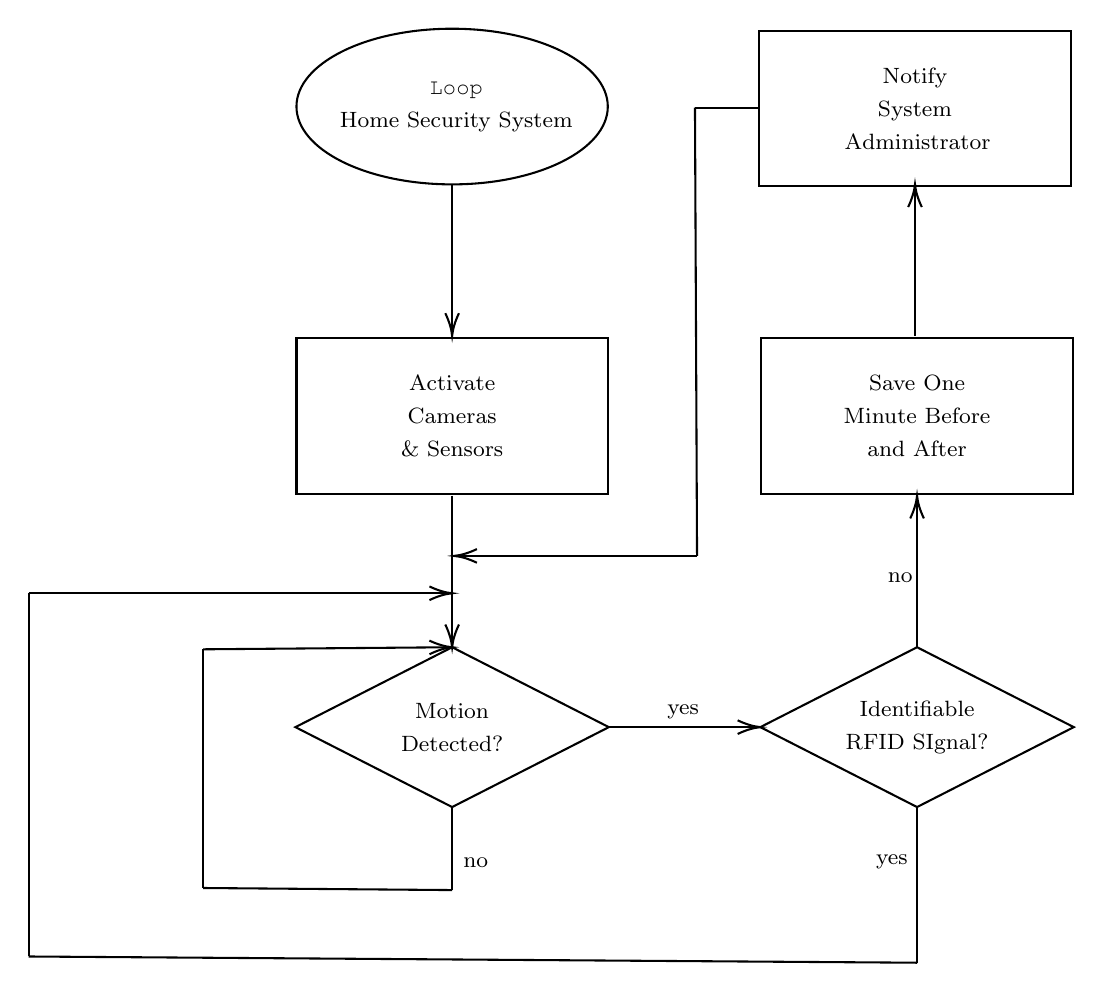
\begin{tikzpicture}[x=0.75pt,y=0.75pt,yscale=-1,xscale=1]
%uncomment if require: \path (0,469); %set diagram left start at 0, and has height of 469

%Shape: Ellipse [id:dp06026735517165571] 
\draw   (248,39.5) .. controls (248,18.79) and (281.58,2) .. (323,2) .. controls (364.42,2) and (398,18.79) .. (398,39.5) .. controls (398,60.21) and (364.42,77) .. (323,77) .. controls (281.58,77) and (248,60.21) .. (248,39.5) -- cycle ;
%Shape: Rectangle [id:dp880516595801381] 
\draw   (248,151) -- (398,151) -- (398,226) -- (248,226) -- cycle ;
%Straight Lines [id:da08375757950130125] 
\draw    (323,77) -- (323,148) ;
\draw [shift={(323,150)}, rotate = 270] [color={rgb, 255:red, 0; green, 0; blue, 0 }  ][line width=0.75]    (10.93,-3.29) .. controls (6.95,-1.4) and (3.31,-0.3) .. (0,0) .. controls (3.31,0.3) and (6.95,1.4) .. (10.93,3.29)   ;
%Flowchart: Decision [id:dp5735470816878454] 
\draw   (323,300) -- (398.5,338.5) -- (323,377) -- (247.5,338.5) -- cycle ;
%Straight Lines [id:da5891435380987948] 
\draw    (323,227) -- (323,298) ;
\draw [shift={(323,300)}, rotate = 270] [color={rgb, 255:red, 0; green, 0; blue, 0 }  ][line width=0.75]    (10.93,-3.29) .. controls (6.95,-1.4) and (3.31,-0.3) .. (0,0) .. controls (3.31,0.3) and (6.95,1.4) .. (10.93,3.29)   ;
%Shape: Boxed Line [id:dp9132377255103166] 
\draw    (398.5,338.5) -- (469.5,338.5) ;
\draw [shift={(471.5,338.5)}, rotate = 180] [color={rgb, 255:red, 0; green, 0; blue, 0 }  ][line width=0.75]    (10.93,-3.29) .. controls (6.95,-1.4) and (3.31,-0.3) .. (0,0) .. controls (3.31,0.3) and (6.95,1.4) .. (10.93,3.29)   ;
%Shape: Rectangle [id:dp6249646563980265] 
\draw   (472,151) -- (622,151) -- (622,226) -- (472,226) -- cycle ;
%Flowchart: Decision [id:dp8409280085137256] 
\draw   (547,300) -- (622.5,338.5) -- (547,377) -- (471.5,338.5) -- cycle ;
%Shape: Boxed Line [id:dp5338753000763605] 
\draw    (547,300) -- (547,229) ;
\draw [shift={(547,227)}, rotate = 90] [color={rgb, 255:red, 0; green, 0; blue, 0 }  ][line width=0.75]    (10.93,-3.29) .. controls (6.95,-1.4) and (3.31,-0.3) .. (0,0) .. controls (3.31,0.3) and (6.95,1.4) .. (10.93,3.29)   ;
%Straight Lines [id:da26354690571623807] 
\draw    (547,377) -- (547,452) ;
%Straight Lines [id:da7739477994676851] 
\draw    (119,449) -- (547,452) ;
%Straight Lines [id:da7947037860822463] 
\draw    (119,274) -- (119,449) ;
%Straight Lines [id:da7385058765120314] 
\draw    (119,274) -- (321,274) ;
\draw [shift={(323,274)}, rotate = 180] [color={rgb, 255:red, 0; green, 0; blue, 0 }  ][line width=0.75]    (10.93,-3.29) .. controls (6.95,-1.4) and (3.31,-0.3) .. (0,0) .. controls (3.31,0.3) and (6.95,1.4) .. (10.93,3.29)   ;
%Straight Lines [id:da8520509248377834] 
\draw    (323,377) -- (323,417) ;
%Straight Lines [id:da69771227917011] 
\draw    (203,416) -- (323,417) ;
%Straight Lines [id:da3020830480387937] 
\draw    (203,301) -- (203,416) ;
%Straight Lines [id:da6539681796101906] 
\draw    (203,301) -- (321,300.02) ;
\draw [shift={(323,300)}, rotate = 179.52] [color={rgb, 255:red, 0; green, 0; blue, 0 }  ][line width=0.75]    (10.93,-3.29) .. controls (6.95,-1.4) and (3.31,-0.3) .. (0,0) .. controls (3.31,0.3) and (6.95,1.4) .. (10.93,3.29)   ;
%Shape: Boxed Line [id:dp4681291110725898] 
\draw    (546,150) -- (546,79) ;
\draw [shift={(546,77)}, rotate = 90] [color={rgb, 255:red, 0; green, 0; blue, 0 }  ][line width=0.75]    (10.93,-3.29) .. controls (6.95,-1.4) and (3.31,-0.3) .. (0,0) .. controls (3.31,0.3) and (6.95,1.4) .. (10.93,3.29)   ;
%Shape: Rectangle [id:dp35495318125677144] 
\draw   (471,3) -- (621,3) -- (621,78) -- (471,78) -- cycle ;
%Straight Lines [id:da33391750072816073] 
\draw    (441,256) -- (326,256) ;
\draw [shift={(324,256)}, rotate = 360] [color={rgb, 255:red, 0; green, 0; blue, 0 }  ][line width=0.75]    (10.93,-3.29) .. controls (6.95,-1.4) and (3.31,-0.3) .. (0,0) .. controls (3.31,0.3) and (6.95,1.4) .. (10.93,3.29)   ;
%Straight Lines [id:da4629225097810108] 
\draw    (471,40) -- (440,40) ;
%Straight Lines [id:da9308190728302066] 
\draw    (440,40) -- (441,256) ;

% Text Node
\draw (325,39.5) node   [align=left] {\begin{minipage}[lt]{85.71pt}\setlength\topsep{0pt}
\begin{center}
{\fontfamily{pcr}\selectfont {\footnotesize Loop}}\\{\footnotesize Home Security System}
\end{center}

\end{minipage}};
% Text Node
\draw (323,188.5) node   [align=left] {\begin{minipage}[lt]{40.36pt}\setlength\topsep{0pt}
\begin{center}
{\footnotesize Activate}\\{\footnotesize Cameras}\\{\footnotesize \& Sensors}
\end{center}

\end{minipage}};
% Text Node
\draw (323,338.5) node   [align=left] {\begin{minipage}[lt]{39.92pt}\setlength\topsep{0pt}
\begin{center}
{\footnotesize Motion }\\{\footnotesize Detected?}
\end{center}

\end{minipage}};
% Text Node
\draw (434.34,336) node [anchor=south] [inner sep=0.75pt]   [align=left] {{\footnotesize yes}};
% Text Node
\draw (547,188.5) node   [align=left] {\begin{minipage}[lt]{53.53pt}\setlength\topsep{0pt}
\begin{center}
{\footnotesize Save One}\\{\footnotesize Minute Before}\\{\footnotesize  and After}
\end{center}

\end{minipage}};
% Text Node
\draw (547,338.5) node   [align=left] {\begin{minipage}[lt]{51.7pt}\setlength\topsep{0pt}
\begin{center}
{\footnotesize Identifiable}\\{\footnotesize RFID SIgnal?}
\end{center}

\end{minipage}};
% Text Node
\draw (546.36,266.5) node [anchor=east] [inner sep=0.75pt]   [align=left] {{\footnotesize no}};
% Text Node
\draw (546.69,403.5) node [anchor=east] [inner sep=0.75pt]   [align=left] {\begin{minipage}[lt]{15.43pt}\setlength\topsep{0pt}
\begin{center}
{\footnotesize yes}
\end{center}

\end{minipage}};
% Text Node
\draw (325,400) node [anchor=north west][inner sep=0.75pt]   [align=left] {\begin{minipage}[lt]{11.8pt}\setlength\topsep{0pt}
\begin{center}
{\footnotesize no}
\end{center}

\end{minipage}};
% Text Node
\draw (546,40.5) node   [align=left] {\begin{minipage}[lt]{50.79pt}\setlength\topsep{0pt}
\begin{center}
{\footnotesize Notify}\\{\footnotesize System}\\{\footnotesize Administrator}
\end{center}

\end{minipage}};


\end{tikzpicture}
